% Include the temperature and pressure history of the cure cycle in the report.
After the layup phase is completed, the curing process can begin. In general, the curing process involves exposing the specimen to high temperatures and pressures. Both the magnitude and duration of the elevated temperatures and pressures influence the quality of the final specimen. Different materials require different cure cycle characteristics for optimal results. A typical cure cycle can be divided in two major steps: the consolidation stage and the cure stage. During the consolidation stage, heat is applied to reach an intermediate temperature and pressure is applied. The heat reduces the viscosity of the resin and the pressure squeezes excess resin out of the laminate. The pressure also "consolidates" the individual specimen plies and removes voids.  During the cure stage, the temperature is elevated even more. The higher temperature initiates resin polymerization and produces crosslinking. 

\begin{figure}[!h]
    \centering
    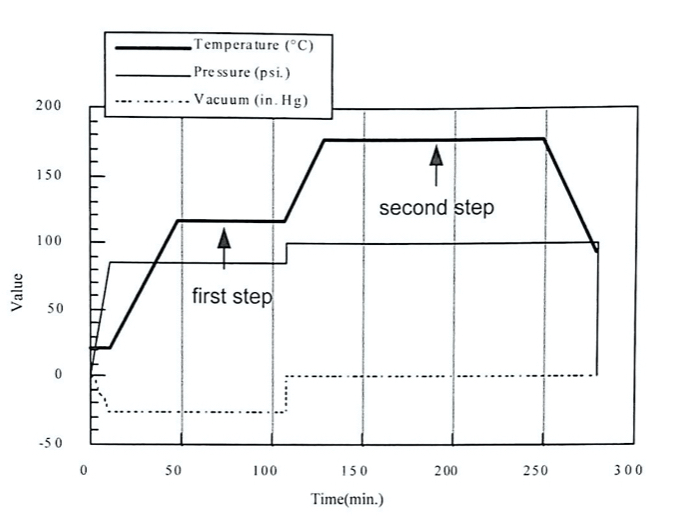
\includegraphics[width=0.65\textwidth]{Pictures/Lab1: Q 1.10/typical_cure.jpg}
    \caption{Typical Cure Cycle\cite{labmanual}}
    \label{fig:typicalcure}
\end{figure}

Figure \ref{fig:typicalcure} displays the temperatures and pressures in a typical cure cycle. Here, the difference in temperatures and pressures between the first and second steps can be seen. 